%%%%%%%%%%%%%%%%%%%%%%%%%%%%%%%%%%%%%%%%%%%%%%
%% Template Thesis DGH UW v3.0
%%
%% Vincent Labatut 04/2015
%% Grégoire Lurton 07/2015
%%
%% v1   - 10/2014 : forme de rapport très différente
%% v2   - 02/2015 : modèle complètement refait
%% v2.1 - 03/2015 : définition de la page de titre
%% v2.2 - 03/2015 : correction de quelques bugs
%% v2.3 - 04/2015 : page de titre complétée (date, adresse postale, long titre)
%% v3.0 - 07/2015 : adaptation de la page de titre pour UW DGH
%% v3.1 - 07/2015 : inclusion de packages pour equations et test pour compilation knitr
%%%%%%%%%%%%%%%%%%%%%%%%%%%%%%%%%%%%%%%%%%%%%%
\documentclass[a4paper,11pt,draft,twoside]{article}

%%%%%%%%%%%%%%%%%%%%%%%%%%%%%%%%%%%%%%%%%%%%%%%%%%%
%% Loading Packages
%%%%%%%%%%%%%%%%%%%%%%%%%%%%%%%%%%%%%%%%%%%%%%%%%%%
\usepackage[english]{babel}
\usepackage[utf8]{inputenc}
\usepackage[T1]{fontenc}
\usepackage{mathpazo}
\usepackage{eulervm}
\usepackage[top=2.5cm, bottom=2.5cm, left=2.5cm, right=2.5cm]{geometry}
\usepackage{setspace}
\usepackage[colorlinks=true , final]{hyperref}
\usepackage[french]{varioref}
\usepackage{lastpage}
\usepackage{fancyhdr}
\usepackage[table]{xcolor}
\usepackage{lmodern}
\usepackage{amsmath,amsthm,amscd,amssymb}
\usepackage{eulervm}

\usepackage{tikz}
\usetikzlibrary{decorations.pathreplacing , chains , intersections}

\usepackage{pgfgantt}
\usepackage{pgfcalendar}





%%%%%%%%%%%%%%
\tikzset{
>=stealth',
  punktchain/.style={
    rectangle,
    rounded corners,
    % fill=black!10,
    draw=black, very thick,
    text width=10em,
    minimum height=3em,
    text centered,
    on chain},
  line/.style={draw, thick, <-},
  element/.style={
    tape,
    top color=white,
    bottom color=blue!50!black!60!,
    minimum width=8em,
    draw=blue!40!black!90, very thick,
    text width=10em,
    minimum height=3.5em,
    text centered,
    on chain},
  every join/.style={->, thick,shorten >=1pt},
  decoration={brace},
  tuborg/.style={decorate},
  tubnode/.style={midway, right=2pt},
}


%%%%%%%%%%%%%%%


\usepackage[numbers]{natbib}
\bibliographystyle{apa-good}

%%%%%%%%%%%%%%%%%%%%%%%%%%%%%%%%%%%%%%%%%%%%%%%%%%%
%% Paper's Information -- TO TWEAK
%%%%%%%%%%%%%%%%%%%%%%%%%%%%%%%%%%%%%%%%%%%%%%%%%%%
%TITLE
\newcommand{\reporttitle}{Methods and Issues for the valorization of HMIS Data}

%AUTHORS
\newcommand{\reportauthors}{Grégoire Lurton}

%PROGRAM
\newcommand{\program}{PhD in Global Health}

%TRACK
\newcommand{\track}{Metrics Track}

%%%%%%%%%%%%%%%%%%%%%%%%%%%%%%%%%%%%%%%%%%%%%%%%%%%
%% Formatting stuff
%%%%%%%%%%%%%%%%%%%%%%%%%%%%%%%%%%%%%%%%%%%%%%%%%%%
\setlength{\headheight}{13.6pt} % due to a warning
\newcommand{\HRule}{\rule{\linewidth}{0.5mm}}
% Espace entre les paragraphes

% Headers and Footers
\pagestyle{fancy}
\fancyhf{}

\renewcommand{\headrulewidth}{0.4pt}
\renewcommand{\footrulewidth}{0.4pt}

\cfoot{\thepage}
\fancyhead[L]{\reporttitle}
\fancyhead[R]{\rightmark}

%%%% Define custom colors
\definecolor{grisclair}{rgb}{0.7,0.7,0.7}
\definecolor{grisfonce}{rgb}{0.5,0.5,0.5}
\definecolor{vert}{RGB}{74,171,67}

%%% PDF Metadatas
\hypersetup{
    pdftitle={\reporttitle},
    pdfauthor={\reportauthors},
    pdfsubject={\reporttitle},
    bookmarksnumbered=true,bookmarksopen=true,
	unicode=true,colorlinks=true,linktoc=all,
	linkcolor=blue,citecolor=blue,filecolor=blue,urlcolor=blue,
	pdfstartview=FitH
}

%%% Font  - Get sans serif
\renewcommand{\familydefault}{\sfdefault}


% Get Bulleted Lists Working
%\renewcommand{\FrenchLabelItem}{\textbullet}

%%%%%%%%%%%%%%%%%%%%%%%%%%%%%%%%%%%%%%%%%%%%%%%%%%
%%% WATERMARK

\usepackage{draftwatermark}
\SetWatermarkText{DRAFT}
%\SetWatermarkScale{5}



\begin{document}
%%%%%%%%%%%%%%%%%%%%%%%%%%%%%%%%%%%%%%%%%%%%%%%%%%%
%% Title Page
%%%%%%%%%%%%%%%%%%%%%%%%%%%%%%%%%%%%%%%%%%%%%%%%%%%
\phantomsection
\begin{titlepage}
	\begin{tikzpicture}[remember picture,overlay]
		\node at (current page.south west)
			{
            \begin{tikzpicture}[remember picture,overlay]
 				\pgftext[x=0cm,y=25.37cm,bottom,left]{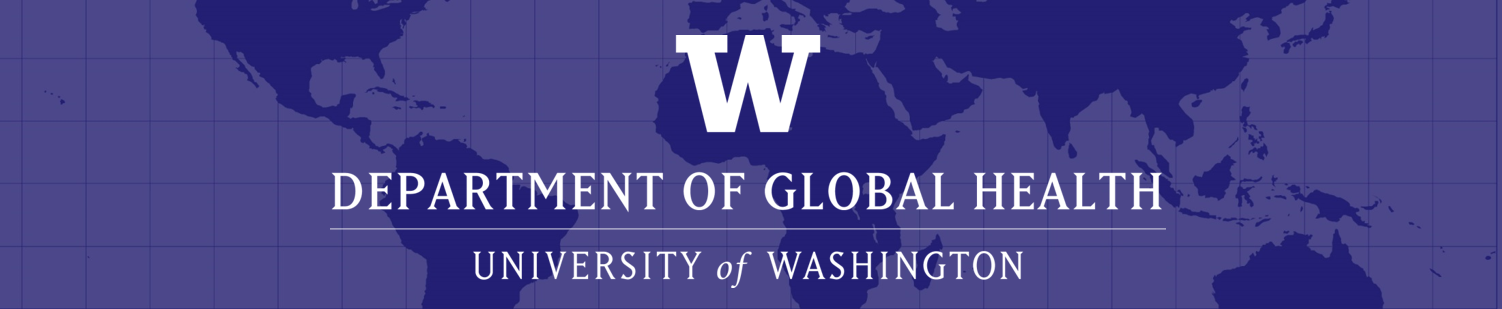
\includegraphics[width=21cm, draft = false]{images/dgh_banner.png}};
 				\pgftext[x=1.1cm,y=24cm,bottom,left]{\fontsize{20}{20}{\textbf{\program}}};
 				\pgftext[x=1.1cm,y=23.2cm,bottom,left]{\fontsize{18}{18}{\textbf{\textcolor{grisfonce}\track}}};
 				\pgftext[x=10.5cm,y=16.5cm,bottom,center]{\fontsize{30}{30}{\textbf{Methods and Issues for }}};%\reporttitle
                \pgftext[x=10.5cm,y=15.2cm,bottom,center]{\fontsize{30}{30}{\textbf{ the valorization of HMIS Data}}};
 				\pgftext[x=10.5cm,y=14.3cm,bottom,center]{\scalebox{0.77}[1]{\fontsize{20}{20}{\fontfamily{phv}\selectfont{}\textcolor{grisfonce}{\reportauthors}}}};
 				%\pgftext[x=5.5cm,y=13.1cm,bottom,left]{\scalebox{0.6}[1]{\fontsize{18}{18}{\fontfamily{phv}\selectfont{}\textbf{\today}}}};
 				\pgftext[x=1.1cm,y=1.8cm,bottom,left]{
\includegraphics[width=6cm , draft = false]{images/ihme_logo.png}};
                \pgftext[x=9.1cm,y=1.8cm,bottom,left]{
\includegraphics[width=6cm, draft = false]{images/itech_logo.png}};
                \pgftext[x=17.1cm,y=1.8cm,bottom,left]{
\includegraphics[width=3cm, draft = false]{images/bluesquare_logo.png}};
                \fill[fill=grisclair] (21cm,1cm) rectangle(0cm,0cm);
	\end{tikzpicture}
				};
			\end{tikzpicture}

\end{titlepage}

%% Get the page after title empty
\pagenumbering{gobble}% Remove page numbers (and reset to 1)
\newpage\null\thispagestyle{empty}\newpage



% TODO Ajouter un DRAFT en surimporession




%%%%%%%%%%%%%%%%%%%%%%%%%%%%%%%%%%%%%%%%%%%%%%%%%%%%%%%%%%%%%%%%%%
%%%%    	FRONT MATTER
%%%%%%%%%%%%%%%%%%%%%%%%%%%%%%%%%%%%%%%%%%%%%%%%%%%%%%%%%%%%%%%%%%
\thispagestyle{plain}
\pagenumbering{roman}
\setcounter{page}{1}



\paragraph{Abstract}

Here the abstract will come

% Table des matières
\cleardoublepage
% Dans le cas du recto verso, ajoute une page blanche si besoin
\phantomsection
\tableofcontents
\addcontentsline{toc}{section}{Table of Content}
\newpage
\addcontentsline{toc}{section}{\listfigurename}
\listoffigures
\newpage
\addcontentsline{toc}{section}{\listtablename}
\listoftables

\thispagestyle{fancy}

% Justification moins stricte : des mots ne dépasseront pas des paragraphes
\sloppy

%%%%%%%%%%%%%%%%%%%%%%%%%%%%%%%%%%%%%%%%%%%%%%%%%%%
%%%% 	MAIN MATTER
%%%%%%%%%%%%%%%%%%%%%%%%%%%%%%%%%%%%%%%%%%%%%%%%%%%

%% Set page numbering right
\cleardoublepage
\pagenumbering{arabic}
\setcounter{page}{1}

\section{Introduction}

\subsection{Motivation}

If a literary form had to be chosen to write or talk about Health Management Information Systems (HMIS), the complaint would probably be everyone's favorite pick. Be it complaints on the burden of work involved in collecting, managing and analyzing data in health systems, or laments on the inexistence of good quality data in most developing countries health systems, HIS are usually described as a non performing burdens of health systems, that can only be improved [HMN citation]. This frustration has multiple causes, and is only matched by the expectations placed in HIS and their widely recognized importance, some authors calling HIS "the foundation of public health"\cite{foundph}. Collecting and analyzing information on activities and results of health systems and on the populations served is indeed essential to guide strategic decision making and to inform health policies.

The complexity of designing and operating well performing national HMIS comes from the fact that HMIS have to handle a high diversity of data and information. Meanwhile, producing this information requires the contribution of a multitude of actors, and is a huge organizational and methodological challenge. Data used to produce relevant health information may come from administrative records, organizational documents or population surveys, and are produced by a variety of actors and organizations, with differing cultures and approaches.
% TODO lister les différents types d'info à produire.

Finally, HIS have to be able to adapt rapidly to changing epidemiological, organizational or political situations. They have to be able to produce relevant information on emerging health issues, and to adapt to the entry of new actors or to a modification in the mode of management of health systems.

In richer countries, the issue surrounding health information is often one of regulation and standardization. The  existence of well performing and well established data sources on populations, and the relative ease of collecting massive amounts of data on individuals pose questions that are mainly related to the protection of privacy, and to the definition of standards for interoperability. The definition of what information should or can be produced is usually a legislative and matter, handled by dedicated entities.

In developing countries, where population data is scarce and data collection can be much more of a challenge, the issues are much different. Health policies depend heavily on the financial, political and technical support of international actors, with differing orientations and priorities. As a consequence, developing countries HIS strengthening programs can be classified into two great families : technology based solutions and institutional reforms. The first family is mainly targeted towards improvement of data collection and relies on solutions relying on the revolution in  data collection capabilities. The second family relies on the adequation of health information produces to policy makers needs, and usually promotes a top-down and normative approach to Information Systems.

If each of these approaches has its benefits and some success stories,  they appear to miss an important part of what makes information systems work. They put their emphasis to the extremes of the information production chains (cf. Figure \ref{HMISFunctions}) and undervalue the middle tiers of these systems. This proposal designs research program oriented towards exploring ways in which this middle tier can be mobilized to improve the value of information produced by HMIS.

This document will start by an introduction of the conceptual framework surrounding the proposed research. We will define Health Management Information Systems, using two classic schematic approaches. We will then define the objectives we will pursue in our research, and will finally describe our different aims and the methods we want to use to complete them.


\section{Conceptual framework}

We will first look at a representation of HMIS through the goals they are meant to fulfill. Once we will have understood why HMIS are used, we will look at a representation of how they are organized.

    \subsection{HMIS definitions}
        \subsubsection{Goal approach}
        \label{sec_goal}

A first approach to HMIS is a consideration of the stated goals of these information systems. Figure \ref{HMISGoals} shows what these main goals are.
\begin{figure}[htp]
\centering
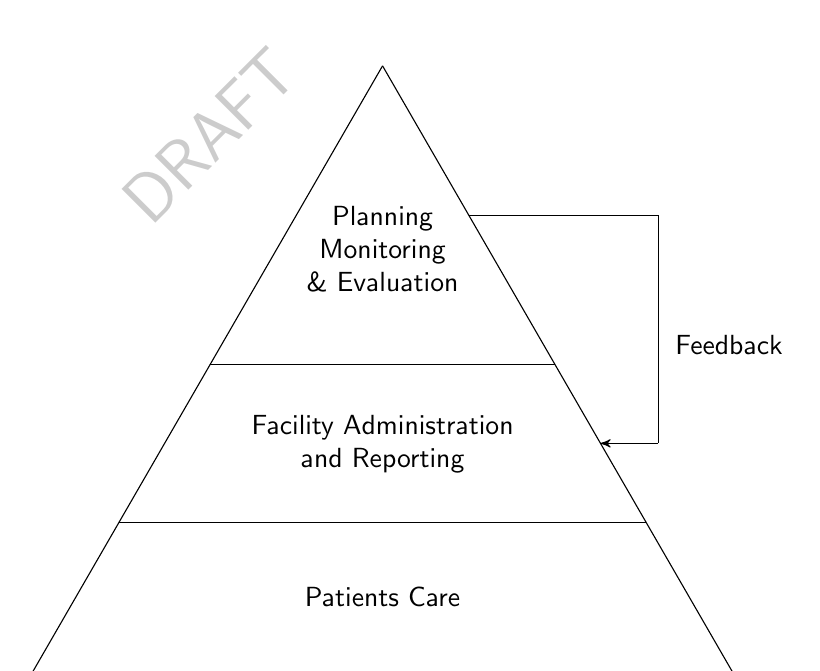
\begin{tikzpicture}[node distance=2cm]
\coordinate (A) at (-4.5,0) {};
\coordinate (B) at ( 4.5,0) {};
\coordinate (C) at ( 0,7.7942) {};
\draw[name path=AC] (A) -- (C);
\draw[name path=BC] (B) -- (C);
\draw (1.1,5.8971)--(3.5,5.8971) ;
\draw(3.5,5.8971)--(3.5,3) ;
\draw [->](3.5,3)--(2.77,3) ;
\node at (4.4,4.25) {Feedback};
\foreach \y/\A/\txtHigh in {0/Patients Care/0.8 ,2/Facility Administration \\ and Reporting/2.5,4/Planning \\ Monitoring \\ \& Evaluation /4.8}{
\path[name path=horiz] (A|-0,\y) -- (B|-0,\y);
\draw[name intersections={of=AC and horiz,by=P},
  name intersections={of=BC and horiz,by=Q}] (P) -- (Q)
  node[align = center,above] at (0,\txtHigh){\A};
  }
\end{tikzpicture}
\caption{Information needs for HMIS}
\label{HMISGoals}
\end{figure}

\begin{description}
\item[Patients Care] Taking care of patients is the primary goal of a health facility. To do so, it is necessary to collect data on these patient, data that will be transmitted (to other services), stored and reused during further follow-ups.
\item[Facility Administration and Reporting] At facility level, HMIS data is used in daily activities to quantify and forecast needs in health inputs, and to create reports for higher levels of the health system.
\item[Planning, Monitoring \& Evaluation] People in charge of the administration of health systems at local or national also need data to monitor activities in the health system, to evaluate the results of interventions, to report to funders or to plan later interventions.
\end{description}

The pyramidal representation of these needs is used to show that these goals fill data needs at different levels of health systems. The different needs for information can roughly thought as being the needs of different type of actors of the health system. Meanwhile, this understanding is not fully true, as at local level, actors will often hold multiple roles and will thus have to use information in different situations. For example, a physician may also be in charge of managing his health facility, and will thus need to plan activities and report on them.



	   \subsubsection{Functional approach}
	    \label{sec_function}

A first way to approach HMIS is to describe the four principal functions that are necessary to have a HMIS to run. Figure \ref{HMISFunctions} presents a simplified sketch of the principal functions that are to be filled in order for HMIS to produce useful information.

\begin{figure}[h]
\begin{center}
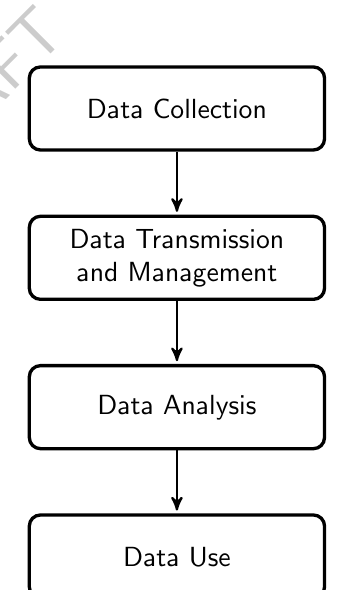
\begin{tikzpicture}[node distance=.8cm,  start chain=going below,]
     \node[punktchain, join] (DataCollection) {Data Collection};
     \node[punktchain, join] (DataManagement) {Data Transmission and Management};
     \node[punktchain, join] (DataAnalysis)   {Data Analysis};
     \node[punktchain, join] (DataUse) 		  {Data Use};
\end{tikzpicture}
\end{center}
\caption{Different functions inside the Health Information Systems}
\label{HMISFunctions}
\end{figure}

\begin{description}
\item[Data Collection] Primary data collection is essential to the production of any information system. In the case of HMIS, data collection happens in health facilities, and is made by health professionals. Data collected in health facilities can be individual patient data collected in patients files or cards. It can also be a first level of aggregation of this data, as for indicators that are reported on a regular basis by facilities to higher levels of the health system. This reporting usually happens through standardized reports, that are then transmitted by successive aggregation to the top of the health pyramid.

\item[Data Management] Data collected in health facilities has to be stored and archived, to be later accessed and reused. Data management work can encompass managing paper data, or managing computerized data. Individual patient data will be computerized in Electronic Medical Records (EMR) whereas aggregated indicators are stored in data-warehouses, like the DHIS2 software.

\item[Data Analysis] Data that is collected and stored in HMIS can then be analyzed. Analysis can be defined as the transformation of data into information. The results of data analysis can be varied, from collection of graphs and maps that can constitute dashboards, to the results of complex models that provide evidences of causality.

\item[Data Usage] Information is the end product of the HMIS, and is used by decision makers or health workers to achieve their tasks. For example, a nurse in a health post may need the monthly consumption of a health product to place an order. A District Health Officer may consider the evolution of monthly number of cases of malaria in his district to plan malaria prevention activities. At national level, a worker at the Ministry of Health may use the number of patients tested positive for HIV to design grant applications for the Global Fund.
\end{description}

Even though the schematic representation of this functions is linear, it should be noted that this linearity is not true in practice. Even once data has been analyzed the results of this analysis has to be archived, and transmitted to the information end users. In some situations, data can be used in its raw form. For example, a physician may use a biological result that he has received in a raw form. Finally, for some data, data collection won't happen inside the health  facility. For example, population survey results may be used to plan and target some interventions, but primary data collection will have happened outside of the health system, and the first function to be used in the HMIS will be the data management function.

The way a program considers and plans each of these functions will define how a specific HMIS will work. We will now present three common approaches to HMIS.

        \subsubsection{Three HMIS archetypes}

Functions of HMIS (cf. section \ref{sec_function}) are not independent of each other. Defining the relative importance of different functions of HMIS in the overall systems can change greatly the way a HMIS functions, and the output it produces. We differentiate three paradigmatic types of HMIS, varying on the respective influence of different functions. Building on the idea that a HMIS is used to provide an image of the activities and performances of a health system, we describe each function as a different way of making an image.

\paragraph{Jigsaw Puzzle HMIS} - A common way to design HMIS in developing countries can be considered as a Jigsaw Puzzle approach. A series of indicators are designed by program managers. These indicators are deemed to be \textit{sensitive} and \textit{specific}, and are supposed to allow managers to track and identify precisely the performance of health systems, and to provide important information on health system's results. The HMIS will then be organized to produce carefully designed indicators at facility level, and to transmit these indicators to higher levels for aggregation.

In these types of system, a lot of importance given to data collection functions, as the quality of this primary data collection is key to the rest of the work in the system. Data management in these system is often limited to aggregating some data and transmitting it to different actors in the health systems. Data analysis is usually mainly descriptive and is limited to presentation of time series values or mapping of indicators along administrative boundaries.

These systems are similar to jigsaw puzzles, made of very specific pieces, to compose a predetermined picture. When they are well designed, these systems can provide very useful information on health systems. Meanwhile, they are very vulnerable to any variation in primary data collection. As for jigsaw puzzles having a piece missing will jeopardize the possibility to get the whole picture right.

\paragraph{Pixel HMIS} - Another way to conceive HMIS is built on the collection and use of a multitude of individual data collected through Electronic Medical Records (EMR). Once the data is collected, program managers can query different indicators on different levels of aggregation, that can be extracted from different EMRs. In the best situations, interoperability of multiple EMRs present in a country allow for a central analysis of the data \cite{pugliese2009large}.

These systems allow a great variety of analysis, with a great variety of approaches. Analysis can be led varying geographic and time focus, or changing definitions of computed quantities. It also allows longitudinal analysis that are more difficult to perform with other approaches.

This approach thus involves a great investment in primary data collection and management, and allows elaborate data analysis. Meanwhile, it requires a technological investment and maturity that is seldom achieved in rich countries, and thus is very rare in developing countries.

\paragraph{Tangram HMIS} - Between the two extremes that are puzzle and pixel HMIS is a third, less prevalent approach to HMIS. This approach will be compared to the tangram game, in which simple forms are used and reused to draw different pictures. In this approach, the emphasis is put on the management functions of HMIS. Simple data elements are collected and stored, and are used and combined in different ways depending on the analysis that is done.

A key component of this model is thus the ability to store and reuse data, thus putting an emphasis on the middle tiers of data management. The use of data warehouses for computerized data is thus a characteristic of this approach. Meanwhile, it also requires an emphasis on data analysis in order to provide relevant information to end users.

    \subsection{HMIS strengthening strategies}

Depending on the HMIS model that is used, programs will implement different type of HMIS strengthening approaches. Programs who privilegy a jigsaw puzzle approach to HMIS will tend to focus on standardizing procedures and methods for data collection and data analysis. Meanwhile, programs who privilegy a pixel approach to HMIS will tend to favour solutions geared towards the implementation of new and performant data collection tools.

\begin{description}
\item[The institutional approach] operates under the assumption that all functions of information systems should be geared towards and submitted to the end information users. This approach tends to be extremely normative as any activity in the information system has to be oriented towards one main predefined goal. In doing so, this approach undervalues the benefits of both the integration of external data, and the positive externalities data collection and analysis may have on multiple users.

\item[The technological approach] relies on the assumption that collecting data and making it available is a sufficient enabler for all other functions of information systems to operate. In this sense, a direct link is made between an information need and a data gap. This approach comes at a cost, and provides only limited benefits if it is not supported by improved data analysis. These solutions tend to provide highly specialized and siloed data collection systems.
\end{description}

We argue these two approaches focus on the most expensive ways to strengthening HMIS (data collection and systemic reforms), and are emphasizing the design of systems and tools that are specific to precisely defined data needs, thus limiting the possibility to implement secondary data usage and the positive externalities of their interventions. The archetype of these pitfalls are the well known parallel and siloed data systems present in many developing countries health systems.

Meanwhile, some of the most significant successes in the strengthening of health information systems in developing countries have been reached precisely through the strengthening of their middle tier. The District Health Information System (DHIS2) project has become a pervasive system to store and organize data collected in developing countries health systems. The DHIS2 approach to health information is based on the organization and storage of multiple data types and sources in a generic data warehousing approach. Its versatility and its ability to adapt to different contexts and data has made it increasingly used in multiple context, thus arguably improving the storage and the availability of health data in low resources countries. Other approaches geared towards the promotion of interoperability of different dimensions of data systems, such as the Open Health Information Exchange framework are also gaining traction.

If these approach have provided efficient solutions to organize and access HMIS data, there is still a lack of solutions to analyze and use HMIS data. Indeed, the high dimensionality of HMIS data and its average low quality make it essentially hard to analyze using standard methods available in developing countries health systems. We will now describe the research project developed to explore ways to analyze this data.


\subsection{Approach and research questions}


This project aims at exploring methods to improve the analysis of HMIS data by using innovative approaches to this data. Using both a technical approach using innovative methods from the data science field, and a critical analysis of health information systems as social objects, we will explore how data currently produced in different health systems can be used and analyzed to produce valuable information. More precisely, we will ask three data main analysis questions :
\begin{itemize}
\item How can metadata collected in an EMR be used in EMR data analysis ?
\item How can different non standardized HMIS sources be mapped and jointly analyzed ?
\item How can multiple data source be integrated to HMIS and analyzed to provide information at local level ?
\item How do decision makers in health systems consider HMIS generated data, and how does it influence the way HMIS are engineered ?
\end{itemize}

Each of these questions explores a different aspect of how standard HMIS data analysis can be expanded to produce useful information with HMIS data. Metadata like the times of creation and savings of EMR forms are indeed seldom used. Meanwhile they provide useful information on how data is collected, and on the working patterns inside health facilities. Our second question explore a different problem, which is often taken as a question of interoperability. Indeed the multiplicity of programs and actors working in many health systems generates a multiplicity of indicators used, that are often related but not identical. There is a need for simple and effective methods to map and conjointly analyze data from different HMIS systems. Finally, HMIS should be useful for local level analysis and decision making. Meanwhile, HMIS data is seldom useful on its own and has to be integrated in larger analysis frameworks to produce interesting information. This integrating can be difficult at national level, but it is even more complicated at local levels, has mapping precisely different data becomes more and more of a challenge at small scale.

We also aim at providing a critical evaluation of the way HMIS are thought of in developping countries societies. Authors like Alain Desrosières and Ted Porter have shown how statistics and computation have come from and generated different cultures of public action in modern societies. The ambivalence of numbers as descriptors or norms has an influence on how information systems are thought of as top-down normative systems instead of knowledge systems. We aim at interrogating how this perception has its roots in long term local historical trends as well as in the tradition and methods of quantitative public health.

To answer these question, we will conduct four distinct research projects.
\begin{description}
    \item[Aim 1] Evaluation of the benefits of improved data collection for HIV patient care in Kenya.
    \item[Aim 2] Test of multiple semantic approaches to interoperability in Bénin.
    \item[Aim 3] Definition and test of a local malaria elimination metric in Namibia.
    \item[Aim 4] Analyze of the theory and practices of Health Information Systems for national decision makers in Mali.
\end{description}

These aims have been designed to provide insights on the problematics posed for each HMIS goal and function. We will now describe each of these aims in more details.


\section[EMR and individual health]{EMR and individual health\footnote{This section is heavily based on KenyaEMR evaluation protocol.}}

A first aim will be to understand how data collection itself impacts quality of care. As we postulate that data collection is not a neutral activity, we want to look into how primary data collected in HIV care setting can impact the outcome of care and organizational capabilities of HIV services. The case we will explore for this project is provided through a project implemented by ITECH in Kenya.

\begin{figure}[ht]
\begin{minipage}{.4\textwidth}
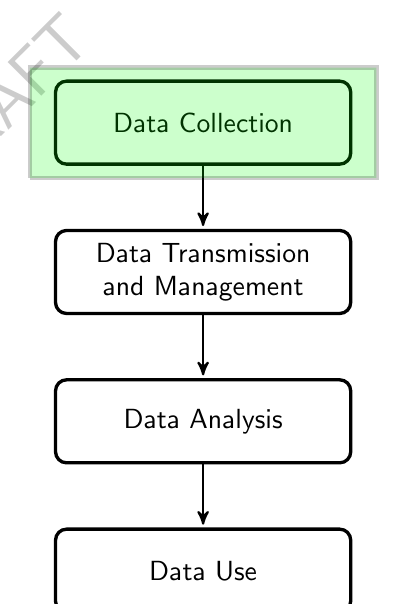
\begin{tikzpicture}[node distance=.8cm,  start chain=going below,]
     \node[punktchain, join] (DataCollection) {Data Collection};
     \node[punktchain, join] (DataManagement) {Data Transmission and Management};
     \node[punktchain, join] (DataAnalysis)   {Data Analysis};
     \node[punktchain, join] (DataUse) 		  {Data Use};
     \filldraw[ultra thick, draw=black, fill=green, opacity=0.2] (-2.2,-.7) -- (-2.2,.7) -- (2.2,.7) -- (2.2,-.7) -- (-2.2,-.7) ;
\end{tikzpicture}
\end{minipage}
\begin{minipage}{.5\textwidth}
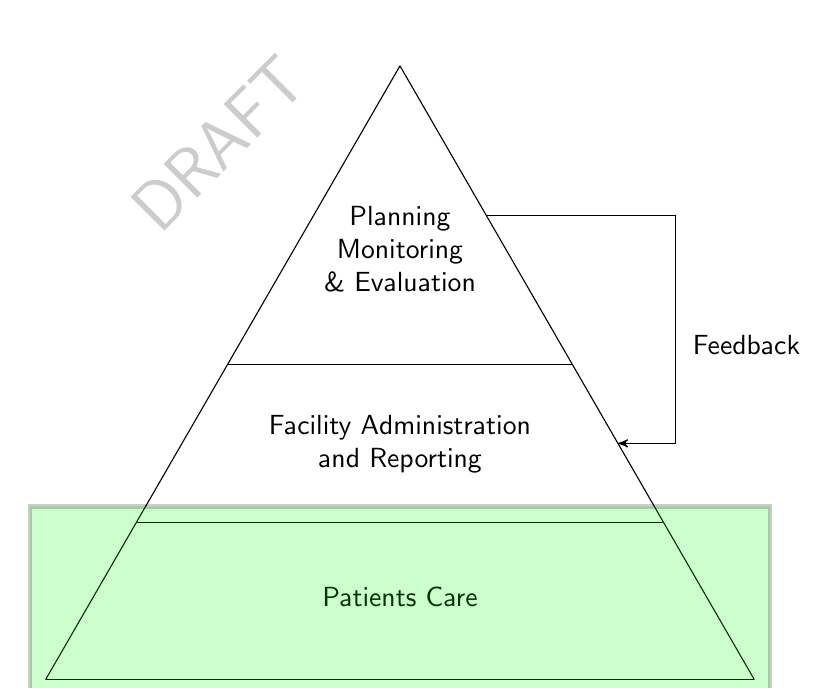
\begin{tikzpicture}[node distance=2cm]
\coordinate (A) at (-4.5,0) {};
\coordinate (B) at ( 4.5,0) {};
\coordinate (C) at ( 0,7.7942) {};
\draw[name path=AC] (A) -- (C);
\draw[name path=BC] (B) -- (C);
\draw (1.1,5.8971)--(3.5,5.8971) ;
\draw(3.5,5.8971)--(3.5,3) ;
\draw [->](3.5,3)--(2.77,3) ;
\node at (4.4,4.25) {Feedback};
\foreach \y/\A/\txtHigh in {0/Patients Care/0.8 ,2/Facility Administration \\ and Reporting/2.5,4/Planning \\ Monitoring \\ \& Evaluation /4.8}{
    \path[name path=horiz] (A|-0,\y) -- (B|-0,\y);
    \draw[name intersections={of=AC and horiz,by=P},
          name intersections={of=BC and horiz,by=Q}] (P) -- (Q)
          node[align = center,above] at (0,\txtHigh){\A};
          }
    \filldraw[ultra thick, draw=black, fill=green, opacity=0.2] (-4.7,-.2) -- (-4.7,2.2) -- (4.7,2.2) -- (4.7,-.2) -- (-4.7,-.2) ;
\end{tikzpicture}
\end{minipage}
\caption{Objective one definition}
\label{Paper One}
\end{figure}


    \subsection{Setting}

In Kenya, I-TECH has implemented an EMR for HIV care, called KenyaEMR, in 341 facilities. The evaluation of this program is currently being carried out. One objective of this evaluation is to assess the effectiveness of KenyaEMR implementation. This effectiveness will be evaluated on two dimensions:

\begin{enumerate}
\item	Improvement of reporting quality in facilities after KenyaEMR implementation
\item	Improvement of quality of care metrics after KenyaEMR implementation
\end{enumerate}

    \subsection{Data}

Kenya’s legal framework for protection of confidentiality of personal health information prohibit transfer of individual patient-level data from any health care facility, even if the data is de-identified. For this reason, the data we will use for this evaluation will be indicators of quality of care, aggregated monthly at facility level, and used for Continuous Quality Improvement (CQI) (see section 4). These indicators will be aggregated on site in Kenya and transmitted for data analysis.

To monitor the maturity of implementation of KenyaEMR (see section 2), we will measure the delay in data entry using metadata stored with KenyaEMR forms, with time stamps for form creation. We will also trace utilization of reporting features of KenyaEMR by using time stamps linked to the use of reports generation. All this data will be extracted and transmitted in raw form for analysis.

To measure the quality of the reports produced for different periods (see section 3), we will consider counts of number of forms entered for a given period, and mean completeness of entered forms. These will be aggregated on site and transmitted for data analysis. We will also use results from Routine Data Quality Assessments (RDQA) that have been conducted in different sites with KenyaEMR implementation. Data for these RDQA are collected in Excel format, and will be used as an external measure of the quality of data entered in KenyaEMR.
In the remaining of this document, we will thus use the following terms:
\begin{itemize}
\item Patient data refers to the data collected by health workers during patients’ visits. They are stored in paper patients’ files, or entered in KenyaEMR forms. We will thus refer to paper patient data or to electronic patient data. This data will not be directly used for analysis in this project.
\item CQI indicators refers to aggregated indicators used to measure quality of care.
\item CQI Report refers to a set of CQI indicators computed for a specific month for a specific facility.
\item DHIS Report refers to the MOH 731 and MOH 711 reports. We will differentiate between paper reports for which the data and the computation of indicators have been made without any digitalization of patients’ data, and electronic reports for which patients’ data has been digitalized. We will be able to use the paper reports as they have been entered in DHIS2 or other data collected by health districts administrations.
\item Patient Forms Metadata refers to the metadata generated by KenyaEMR when patient forms are entered. The metadata used should mainly be timestamps related to time of data entry.
\item Reporting Metadata refers to timestamps generated by KenyaEMR when different types of report are generated.
\item RDQA Data refers to raw data collected during RDQA exercises.
\end{itemize}

    \subsection{Implementation maturity}

We distinguish three different periods in the implementation of the EMR. Each of these periods is characterized by different ways the data is collected, entered, analyzed or used. For each of these periods, we will also have access to different types of data. We will describe the characteristics of each of these periods, and present a strategy to categorize the available data in each of these periods, using DHIS and CQI reports and metadata.

        \subsubsection{Paper Based}

In the first period, no patient data entry is made in the facility. Patient data is collected in paper files, and reports are computed manually using these files. In the meantime, health workers can only use paper data to follow their patients.

The data we will be able to access from this period is:
\begin{itemize}
\item	The patient data that will have been retrospectively entered in KenyaEMR
\item	The paper reports that will have been entered in DHIS2 or other reports available from health districts administrations
\end{itemize}

        \subsubsection{Retrospective Data Entry}

In a second period, data entry has been implemented in the facility. The backlog of paper patient data has to be retrospectively entered, and current patient data is also entered in KenyaEMR after a delay. During this period, health workers will still refer to paper data to follow their patients. This is the Routine Data Entry phase (RDE).

The data we will be able to access from this period is:
\begin{itemize}
\item	The patient data entered in KenyaEMR
\item	The metadata for patient data entered in KenyaEMR
\item	The CQI and DHIS reports computed from this data
\item	The reporting data metadata
\item	Evaluations of data quality from RDQA
\end{itemize}

        \subsubsection{Point of Care}

In a third period, the patient data is entered either by the health worker or by a specialized data clerk based on patient data collected on paper by the health worker, in quasi real time with the medical consultation. We call this phase the Point of Care (POC) phase.

The data we will be able to access from this period is:
\begin{itemize}
\item	The patient data retrospectively entered in KenyaEMR
\item	The metadata for patient data entered in KenyaEMR
\item	The CQI and DHIS reports computed from this data
\item	The reporting data metadata
\item	Evaluations of data quality from RDQA
\end{itemize}

        \subsubsection{Transition periods}

There may be some overlaps between different periods. For example, the limit between the paper collection and routine data entry may not be clear cut, as some facilities may have tried to start entering more recent patient forms during the RDE period, to be on top of the work quickly. Similarly, some facilities may have been at the same time doing retrospective data entry for some forms, and POC data entry for some others, depending on the organization of care.

To take this into account, we will need to consider overlapping periods for different aspects of the data.
\begin{itemize}
\item	Data quality: the process to collect and enumerate patient data is identical in paper based period and RDE period. Meanwhile, in the POC period, data is possibly directly entered in KenyaEMR, without using a paper form. Also, rapid data entry may allow to go back to the HW to complete missing data, or to correct unclear information.
\item	Report computation quality: Once the data entered in KenyaEMR, the reports can be computed automatically. Thus, the quality of computation of reports will be identical in POC and RDE, but will likely differ from the Paper Based period (see Section 3 for more details on Reporting Quality).
\item	Quality of care: in the paper based period as in the RDE period, HW can only access patient data through paper files. They thus can’t use automated reminders, or summary information offered by KenyaEMR. Meanwhile, starting in the RDE period, some reports can be edited through Kenya EMR that would allow health worker to better track late and defaulting patients, and thus would allow them to pass reminders calls, or plan lab tests. We would thus anticipate to see a slightly improved quality of care for RDE period compared to Paper Based period, and to see an additional improvement for POC period compared to RDE period.
\end{itemize}

Table 1 presents a summary of the different periods described. Based on this periodization, we will want to test three main hypothesis:
\begin{enumerate}
\item	Observed data quality is similar in paper and RDE period, and better in POC period.
\item	Computation quality is bad in paper-based period but then improved in RDE and POC periods.
\item	Quality of care is worst in paper-based period, improves in RDE and is best in POC period.
\end{enumerate}


%	Paper Based	RDE	POC
%Data Collection	Paper Based	Paper Based	Computer Based
%Data Entry	No	Retrospective	Real Time
%Data Analysis	Paper Based	Computer Based	Computer Based
%Data Use	Paper Based	Paper Based	Computer Based

%Data Quality	Stage 1	Stage 2
%Computation Quality	Stage 1	Stage 2
%Quality of care	Stage 1	Stage 2	Stage 3
%Table 1 - Different period of implementation and stages of evaluative outcomes

        \subsubsection{Methods for periodization}
For each facility included in this analysis, we will have to define when they enter or exit each of these periods. To do this, we will use programmatic data collected by I-TECH staff to monitor the implementation of KenyaEMR, and time stamps associated with forms entered in KenyaEMR, and Building on the characteristics of the different periods, we will categorize the different dimensions of the data collection and use separately:

\begin{enumerate}
\item    Data Quality: The passage between stage 1 and stage 2 of data collection will be tracked looking at the delay of data entry of forms. Looking at the distribution of this delay, and using I-TECH monitoring data for confirmation, we will define a threshold to define stage 2 data entry. We will also use comparison of data completeness between different periods.
\item	Report Computation: The passage between stage 1 and stage 2 of report computation will be tracked looking at the source of the reports available for the facility. Existence of reports from DHIS2 or similar source that were not produced using KenyaEMR computation will lead to the categorization of the stage of report computation as stage 1. Reports computed with KenyaEMR will lead to a categorization of the period as a stage 2 for report computation. The categorization will be validated with data from I-TECH monitoring, and by a comparison of results reported in DHIS2 and results computed for the same month from KenyaEMR.
\item	Data usage: The passage between stage 1 and stage 2 for data usage will be used considering metadata from different reports, and delay of data entry. A different threshold as the one used for data quality will be used to categorize a facility as stage 1 or 2 for quality of care.
\end{enumerate}

Using available data to explore this different dimensions, we will be able to categorize each facilities’ reports into its corresponding period. As we anticipate some exceptions due to unclear transition periods, we will design a continuous index of maturity of implementation of KenyaEMR, to be included in latter stages of the analysis. Depending on the results of the exploratory work, we will use a continuous index or a discrete periodization of the intervention.

\subsection{Reporting quality}
To estimate the impact of KenyaEMR on the quality of reporting, we will compare aggregated monthly reports on HIV activities in facilities produced before and after implementation of KenyaEMR. Evolution of reporting quality involves two evolutions: amelioration of primary data quality, and amelioration of report computation quality.


%%Figure reporting Quality

We will measure data quality by looking at specific metrics:
\begin{itemize}
\item	Proportion of data fields used to compute reports that have contain valid data
\item	Mean monthly number of visits by active patients
\end{itemize}

We will also use RDQA data to evaluate the quality of the data. Using RDQA results as training results, we will explore systematic classification of data quality based on reports indicators and patient forms metadata distribution.

We will then measure the evolution of data quality between RDE and POC data in KenyaEMR and we will perform simple comparisons to evaluate changes in data quality when entering data directly in computerized form.

Also, we expect computation quality to have multiple measurable impacts:
\begin{itemize}
\item	Greater coherence of indicators involving longitudinal data analysis,
\item	Greater coherence of indicators involving multiple data sources
\item	Greater coherence of indicators evolution in time, as computerized computation will be exactly the same in time
\item	Greater coherence of indicators between facilities, as computerized computation will be exactly the same in all facilities.
\end{itemize}

We will compare reports generated for the same facilities and same months, in Period 1 and Period 2, and we will perform simple comparisons to evaluate changes when using standardized computation methods.

Based on these two dimensions of reporting quality, we will finally design an index of reporting quality that will be used in subsequent analysis. Quality of reporting will then be modelled using, using facility characteristics as covariate, and the index of maturity of implementation. The coefficient associated to maturity of implementation will be considered as the measure of the impact of KenyaEMR on reporting quality (see section Quality of Care and patient health outcome4 for presentation of the modeling strategy).

\subsection{Quality of Care and patient health outcome}

Using existing aggregate-level longitudinal data from KenyaEMR sites, we will retrospectively compare quality of care and patient health outcome indicators during each period of the EMR transition. The specific quality of care and patient health outcome indicators to be examined will be determined in collaboration with CDC and the MOH, based on commonly-used indicators within Kenya and globally. A list of these indicators can be found in Annex C.

To model the association between using KenyaEMR and the level of each quality of care and patient health outcome indicators, we will use Generalized Estimating Equations (GEE) that will allow us to take into account the temporal correlation of observations. Covariates that we will introduce in this model include:
\begin{itemize}
\item	Facility type
\item	KenyaEMR implementation maturity index
\item	Reporting quality index
\item	Number of patients followed for HIV in the facility
\item	Number of HW involved in HIV care in the facility
\item	Time trend
\end{itemize}
The coefficient estimated for KenyaEMR implementation maturity index in this model will be considered as the measure of the impact of KenyaEMR on the quality of care and the health outputs of HIV patients. The index will be introduced in continuous form or in dichotomized form. Alternative proxy of KenyaEMR implementation will also be tested such as period of implementation as defined for quality of care in table 1.

\subsection{Timeline} Figure XX presents a timeline for the realization of this objective. Even though the data collection process could be a sort of blackbox, we expect this paper to be finished by DDDD.

\begin{figure}[h]
\begin{ganttchart}[vgrid,hgrid]{1}{24}
\gantttitle{2016}{12}
\gantttitle{2017}{12} \\
\gantttitlelist{1,...,12}{1} \gantttitlelist{1,...,12}{1}\\
%\ganttgroup{Group 1}{1}{7} \\
\ganttbar{Data Extraction}{1}{3} \\
\ganttbar{Data Cleaning}{2}{4} \\
\ganttbar{Data Analysis 1}{5}{6} \\
\ganttmilestone{Sharing First Results}{6} \\
\ganttbar{Data Analysis 2}{7}{9} \\
\ganttmilestone{Sharing Final Results}{9} \\
\ganttbar{Paper Writing}{9}{11} \\
\ganttmilestone{Paper Submission}{11}
\end{ganttchart}
\caption{Gantt Chart for Paper 1}
\end{figure}


\section{Semantic analysis and grouped analysis}

The second approach of this dissertation regards the management of data collected in hospitals in developing countries. Many systems have been developed to store this data and use it in different situations. Meanwhile, some problems are frequently found, that prevent statisticians and public health scientists to use this data. Issues regarding data completeness and data quality are of primary importance. An issue regarding these questions is the lack of validation frameworks for data systems. Data coming from one system is seldom confronted, or even less validated with data from a different system. As a result, monitoring and definition of data quality is usually mainly a procedural concept for data producing entities, and a critical and often restrictive aspect of data analysis.

We aim at offering a set of methods that allow the use of different existing data sources in order to enforce better data quality and data completeness. This entails two main aspect :

\begin{enumerate}
\item A framework for interoperability of different data systems
\item A framework for validation of data
\end{enumerate}

\begin{figure}[ht]
\begin{minipage}{.4\textwidth}
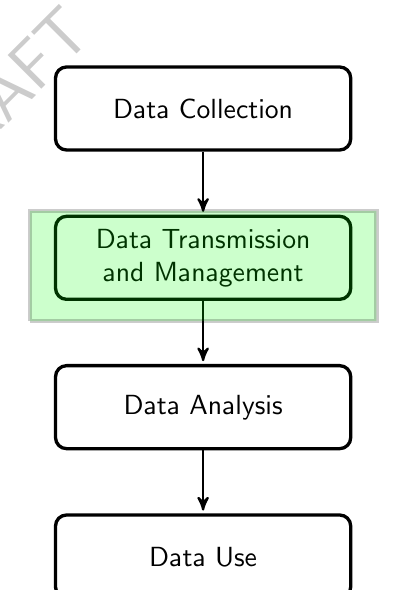
\begin{tikzpicture}[node distance=.8cm,  start chain=going below,]
     \node[punktchain, join] (DataCollection) {Data Collection};
     \node[punktchain, join] (DataManagement) {Data Transmission and Management};
     \node[punktchain, join] (DataAnalysis)   {Data Analysis};
     \node[punktchain, join] (DataUse) 		  {Data Use};
     \filldraw[ultra thick, draw=black, fill=green, opacity=0.2] (-2.2,-2.7) -- (-2.2,-1.3) -- (2.2,-1.3) -- (2.2,-2.7) -- (-2.2,-2.7) ;
\end{tikzpicture}
\end{minipage}
\begin{minipage}{.5\textwidth}
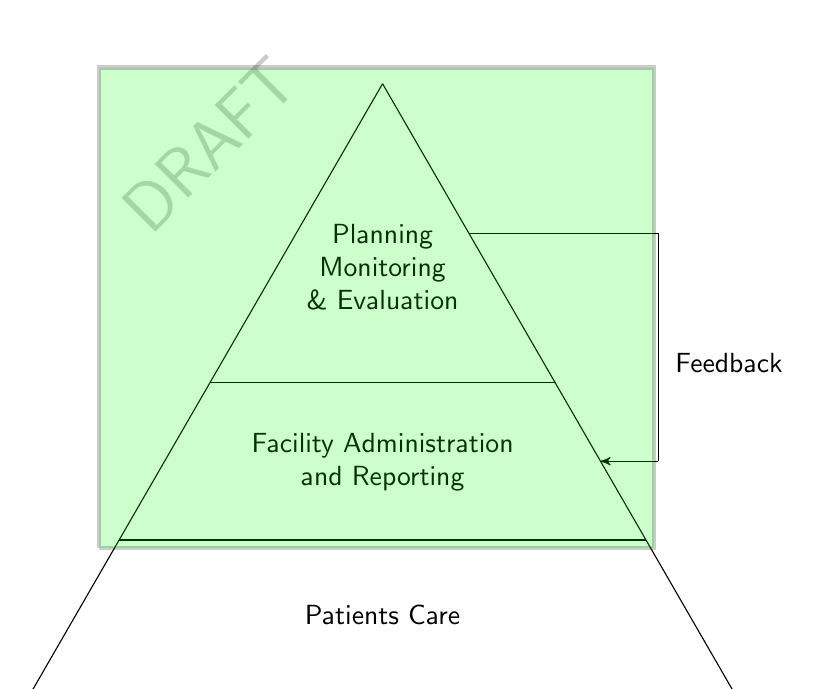
\begin{tikzpicture}[node distance=2cm]
\coordinate (A) at (-4.5,0) {};
\coordinate (B) at ( 4.5,0) {};
\coordinate (C) at ( 0,7.7942) {};
\draw[name path=AC] (A) -- (C);
\draw[name path=BC] (B) -- (C);
\draw (1.1,5.8971)--(3.5,5.8971) ;
\draw(3.5,5.8971)--(3.5,3) ;
\draw [->](3.5,3)--(2.77,3) ;
\node at (4.4,4.25) {Feedback};
\foreach \y/\A/\txtHigh in {0/Patients Care/0.8 ,2/Facility Administration \\ and Reporting/2.5,4/Planning \\ Monitoring \\ \& Evaluation /4.8}{
    \path[name path=horiz] (A|-0,\y) -- (B|-0,\y);
    \draw[name intersections={of=AC and horiz,by=P},
          name intersections={of=BC and horiz,by=Q}] (P) -- (Q)
          node[align = center,above] at (0,\txtHigh){\A};
          }
    \filldraw[ultra thick, draw=black, fill=green, opacity=0.2] (-3.6,1.9) -- (-3.6,8) -- (3.45,8) -- (3.45,1.9) -- (-3.6,1.9) ;
\end{tikzpicture}
\end{minipage}
\caption{Objective two definition}
\label{Paper Two}
\end{figure}

\subsection{Interoperability framework}

% IDEA Interoperability different dimensions : concentration on semantic and validation on analysis

POINT SUR INTEROPERABILITY BRAA / SAHAY / EXPLICATION TRAVAIL DEJA FAIT

Our aim will be to define and test these two frameworks, building on some work currently happening around interoperability frameworks. In this project, conducted with health information startup Bluesquare, we aim at defining a tagging based approach to interoperability. With this approach, each health service indicator in a given facility reporting framework is defined based on three dimensions : health issue, population target and type of service provided. A first level of testing has already implemented in Bénin, matching DHIS2 indicators with OpenRBF indicators. Using this simple method, it was possible to match correctly XX\% of GG indicators from the OpenRBF framework with a subset of YY\% indicators from the DHIS2 framework.

One of the biggest benefits of this approach is its ability to define a notion of \textit{distance} between indicators. Indicators that related by one dimension will be farther apart from each other than indicators that are related by two dimensions. Also, for dimensions that are not defined on a discrete basis (for example age boundaries for a population), incomplete correspondence can be quantified.

Building on this flexibility, it is possible to automatically map datasets between each other, and to offer possibilities of joint analysis between data sets. A first level of analysis is the validation of data, informed by comparison of different data sets.

Used for data validation, imputation / completion.


\subsection{Research questions}

DEFINITIONS ON DATA VALUES AND OTHER RELATED CONCEPTS

\begin{enumerate}
\item Define and test an algorithmic approach to assert data credibility from a given data set
\item Define and test an approach to compare and complete data missingness using imputation and external data
\end{enumerate}

\begin{enumerate}
\item What is the performance of different approaches
\item What is a good metric to assert data quality and completeness of a given data set
\item What is a good metric to assert comparability of two indicators or data sets.
\end{enumerate}

\subsection{Validation framework}

Our main aim will be to gauge the credibility of a data value or of a dataset.  We can anticipate different situation we would like to investigate :
\begin{description}
\item[simple outlier] are situations when an isolated data value in a dataset is wrong, for one facility once. These are the situations that are the most commonly considered outliers. This may be the most straightforward situation.
\item[outlying report] are situations when all values of one report appear to be off. This may be due to an update in the tools or methods for some indicators, or to the training of a new Health Worker in the facility who does not fully comply with usual ways to compute indicators.
\item[outlying facility] are situations when one facility is consistently reporting numbers that are different from surrounding facilities. This may happen when structural conditions in one facility are leading to discrepancies in data collection, or in data computation.
\end{description}

We want to attach to each value a probabilistic value for the credibility of a data value, or of a data set. The combination and comparison of the credibility of multiple data points or reports at multiple levels in turn gives a fine grained picture of data credibility, and orients actions to be taken.

%% ie ce qu'on propose n'est pas orienté pour corriger les données mais pour construire un meilleurs système par la suite. Plus orienté développement et value l'utilisation des données plus que leur perfection. Imputation pour données fausses.

The data validation work will be conducted using data from OpenRBF Bénin, with data values entered and verified being recorded.

\paragraph{Estimation} Multiple models

\paragraph{Description} Dashboarding

\paragraph{Decision} Decision

Using the validation dataset from OpenRBF, we will try and predict error using a simple predictive approach bagging different Machine Learning Classification methods. Result of this approach will be a probabilistic assessment of data quality for each indicator value. This, in turn, will be turned in a facility level dashboard, tracking estimated quality of reporting in time. A district level dashboard could also be created, to track average data quality in different districts.

In predicting data validity, we will test the introduction of weighting of different predictors, based on their estimated distance from a given indicator. This will be made for each indicator, internally and externally, and testing different definitions of inter-indicator distance.

Finally, we will use similar methods as previously to impute true values of missing or false indicators. Validation of these will be made using standard validation techniques (k-Fold, etc...)

\subsection{timeline}

Figure XX presents a timeline for the realization of this objective. Even though the data collection process could be a sort of blackbox, we expect this paper to be finished by DDDD.

\begin{figure}[h]
\begin{ganttchart}[vgrid,hgrid]{1}{24}
\gantttitle{2016}{12}
\gantttitle{2017}{12} \\
\gantttitlelist{1,...,12}{1} \gantttitlelist{1,...,12}{1}\\
%\ganttgroup{Group 1}{1}{7} \\
\ganttbar{Data Extraction}{1}{3} \\
\ganttbar{Data Cleaning}{2}{4} \\
\ganttbar{Data Analysis 1}{5}{6} \\
\ganttmilestone{Sharing First Results}{6} \\
\ganttbar{Data Analysis 2}{7}{9} \\
\ganttmilestone{Sharing Final Results}{9} \\
\ganttbar{Paper Writing}{9}{11} \\
\ganttmilestone{Paper Submission}{11}
\end{ganttchart}
\caption{Gantt Chart for Paper 2}
\end{figure}

\section{Innovative analytic approach - data integration for malaria elimination}

% TODO here, integration of the GCE proposal. Not precise on geography yet.

HMIS data is most often very highly dimensional. A high number of indicators is collected on a regular basis in a host of facilities. Classic data analysis methods used in Public Health are not always suited to explore this type of data, especially due to the average low quality and completeness of the data. We aim at defining methods that can help make better use of this type of data for policy and decision making purposes. Mainly, we want to orient our work on reducing dimensionality of the HMIS data for analysts and policy makers.

A consequence of this is that policy makers usually concentrate on issues that are not dictated by what they see in their own data but concentrate on issues dictated at higher, national or international levels. This is akin to the classic story of the economist looking for his keys under a lamppost while he lost them somewhere else. Analysis is only directed at variables for which there is external light.

Reducing dimensionality may come in different ways. Most important ones we have easy access to are :

\begin{itemize}
\item Reduce interesting indicators
\item Reduce organizational unit to concentrate on
\item Reduce data values to concentrate on
\end{itemize}

Building on literature of quality control in the industrial realm, we want to define observed norms and standards and simply identify units that differ from these norms and standards.


1. Indicator wise standardization
2. Spatial smoothing and validation
3. Temporal modeling and validation



\begin{figure}[ht]
\begin{minipage}{.4\textwidth}
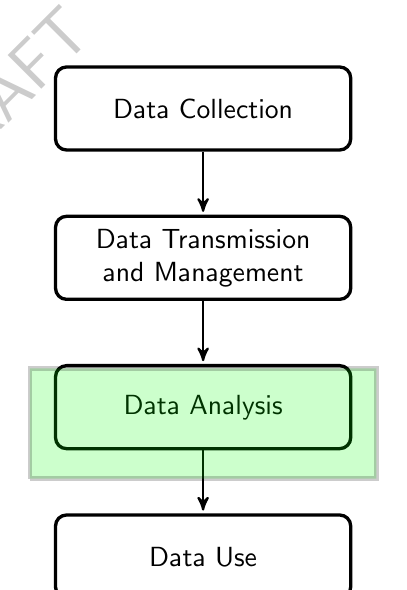
\begin{tikzpicture}[node distance=.8cm,  start chain=going below,]
     \node[punktchain, join] (DataCollection) {Data Collection};
     \node[punktchain, join] (DataManagement) {Data Transmission and Management};
     \node[punktchain, join] (DataAnalysis)   {Data Analysis};
     \node[punktchain, join] (DataUse) 		  {Data Use};
     \filldraw[ultra thick, draw=black, fill=green, opacity=0.2] (-2.2,-4.7) -- (-2.2,-3.3) -- (2.2,-3.3) -- (2.2,-4.7) -- (-2.2,-4.7) ;
\end{tikzpicture}
\end{minipage}
\begin{minipage}{.5\textwidth}
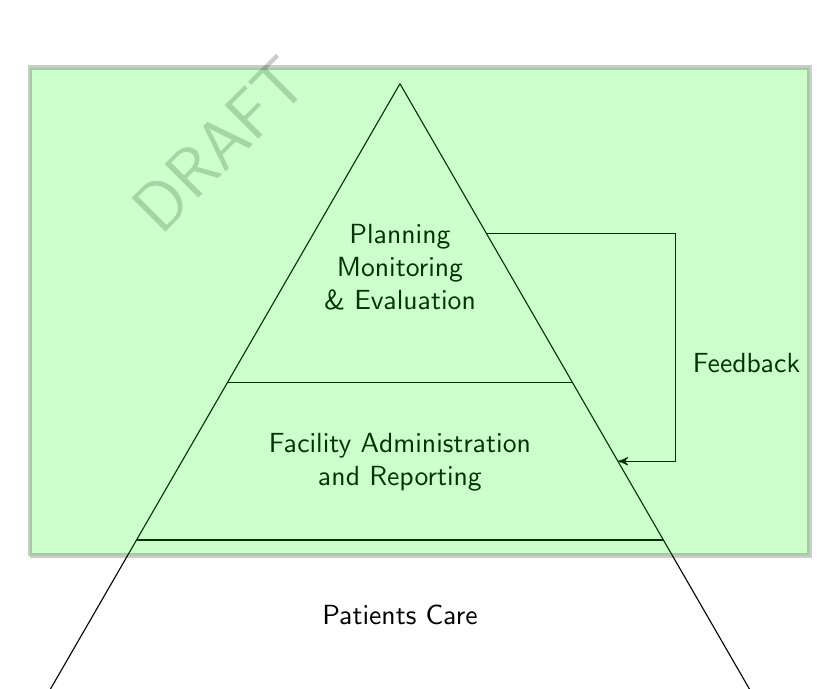
\begin{tikzpicture}[node distance=2cm]
\coordinate (A) at (-4.5,0) {};
\coordinate (B) at ( 4.5,0) {};
\coordinate (C) at ( 0,7.7942) {};
\draw[name path=AC] (A) -- (C);
\draw[name path=BC] (B) -- (C);
\draw (1.1,5.8971)--(3.5,5.8971) ;
\draw(3.5,5.8971)--(3.5,3) ;
\draw [->](3.5,3)--(2.77,3) ;
\node at (4.4,4.25) {Feedback};
\foreach \y/\A/\txtHigh in {0/Patients Care/0.8 ,2/Facility Administration \\ and Reporting/2.5,4/Planning \\ Monitoring \\ \& Evaluation /4.8}{
    \path[name path=horiz] (A|-0,\y) -- (B|-0,\y);
    \draw[name intersections={of=AC and horiz,by=P},
          name intersections={of=BC and horiz,by=Q}] (P) -- (Q)
          node[align = center,above] at (0,\txtHigh){\A};
          }
    \filldraw[ultra thick, draw=black, fill=green, opacity=0.2] (-4.7,1.8) -- (-4.7,8) -- (5.2,8) -- (5.2,1.8) -- (-4.7,1.8) ;
\end{tikzpicture}
\end{minipage}
\caption{Objective three definition}
\label{Paper Three}
\end{figure}

    \subsection{Setting}

    \subsection{Data}

    \subsection{Analysis}

    \subsection{Timeline}


\section{Data Use}

construction d'un espace politique d'équivalence et de codage


"Les outils statistiques permettent de découvrir ou de créer des êtres sur lesquels prendre appui pour décrire le monde et agir sur lui" - citation sur la decision rationnelle. mais on sait que c'est un construit. Social et technique. Cas spécifique, statistique sanitaire



\subsection{Information in Health Systems}

The use of statistical information for the management of complex organizations has evolved since the beginning of the XIX\th century. Since the invention of population by XVIII\th century demographers[DESROSIERES], and the integration of numbers in the political and administrative language in the second XIXth century (PORTER), multiple types of information have been used for the orientation of public policies and the administration of public services. Meanwhile, the rise of epidemiology and the critalization of a body of knowledge around the institutions in charge of the defense of Public Health helped creating a specific Public Health oriented spin on quantitative information for health systems [BIBLIO]. The needs for information and data thus are varied at different levels of health systems

Finally, recognizing even an excellent technical framework can not ensure the proper use of statistical information in a health system, we want to reflect on the culture of data use in developing countries health systems. To do so, we want to adopt a post colonial approach, and understand how a vision of statistics resulting from colonial rule and neo-liberal management results in a deficit of data using for health systems related decisions.


The use of data for public decision is consubstantial to the apparition and the development of public as a domain of public action. The "invention of population" in the second half of the XVIIIth century was made possible by the reform and development of demographic information in Europe and the development of demographic methods. In later stages, the development of sampling and inferential statistics methods in the XIXth century was also key to the targeting of specific public health interventions.

The use of data for policy making is thus, as we see, a combination of data sources, statistical methods, and political or social norms, that will define the conditions of utilisation of statistical evidence for policy making. Finding the proper data source, being able to analyze it and incorporating the results of this analysis in a political process is essential to the proper use and utilization of information systems.

In Global Health realm, the use of data for the definition of \textit{evidence based} intervention and policies has emerged as a panacea of project design and management. There are nonetheless difficulties in this regard. The global nature of public health means that statistical data available for analysis is by nature scattered and varied in nature, technical characteristics, quality and scope. In the meantime, the exigence of Global Health practitioners is to use and understand varied data sources in a unified global framework. The Global Burden of Disease initiative is a good example of this exigence of a global assessment of a wide variety of data from multiple contexts.

The challenge of using and processing different kinds of data varies with the nature of the data sources. The design and definition of survey data, for example, is governed by methodological and technical constraints that are comparable between settings and implementations. Meanwhile, data from health systems will be influenced by multiple factors, ranging from the administrative traditions in which they develop, to the level of resources involved in the design and building of these data systems, and to the type of activities performed in these systems. Among them, hospital data could arguably be considered the most impacted by these different factors.

\subsubsection{The administrative legacy}

There has been a long term evolution since the early XIX\th century as of how data should be produced and used in health systems. As


reductio ad M\&E


Question de la statistique coloniale. Les différents niveaux de la statistique administrative, importance de la justification et du contrôle dans l'utilisation faites des données administratives.

There is a primary problem in the use of HMIS data. Alain Desrosières has shown the richness and complication of the production and use of statistics in modern societies. Desrosières shows how two traditions have been cohabiting in the early ages of the production of social statistics\cite{admin_savant}.

\begin{quote}
The first tradition is administrative, and is based on political science and the law, on the German Staatenkunde, from the time of Conring and Achenwall. It is more taxonomic than metrological: it is designed to classify facts systematically rather than measure them, which is the essence of the other tradition, the "English" tradition. The latter, inspired more by the natural sciences and by progress made in measurement and probability theories, is a distant relation of the English political arithmetic of Graunt and Petty.
\end{quote}

Desrosières later shows how these two traditions have bee reconciled in the modern figure of the statistician, at the same time administrator and scientist. It is useful to keep considering this tension when thinking about maturing statistical systems like developing countries' HMIS. Being able to distinguish between situations when actors of HMIS are acting as administrators, and when the position is that of a metrician is essential to understand HMIS issues and offer informed solutions.

This distinction is essential at many levels. The whole debate around the level of uncertainty that is bearable around a measurement is not only important for statisticians. Choosing a given approach will have an impact on how primary data will be collected, how it will be analyzed, and how it will be used. In many usages of HMIS, complete enumeration is deemed necessary, but this can be discussed. What is the level of confidence one can bear around the estimation of a stock of drugs ?

In other dimensions, how can civil society help for HMIS design and evaluation

M\&E = version la plus degradee

\begin{figure}[ht]
\begin{minipage}{.4\textwidth}
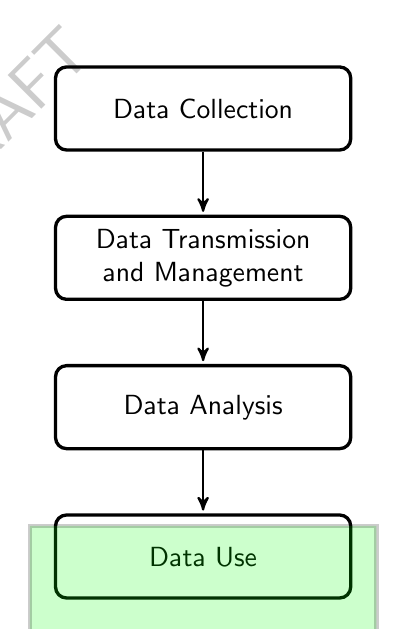
\begin{tikzpicture}[node distance=.8cm,  start chain=going below,]
     \node[punktchain, join] (DataCollection) {Data Collection};
     \node[punktchain, join] (DataManagement) {Data Transmission and Management};
     \node[punktchain, join] (DataAnalysis)   {Data Analysis};
     \node[punktchain, join] (DataUse) 		  {Data Use};
     \filldraw[ultra thick, draw=black, fill=green, opacity=0.2] (-2.2,-6.7) -- (-2.2,-5.3) -- (2.2,-5.3) -- (2.2,-6.7) -- (-2.2,-6.7) ;
\end{tikzpicture}
\end{minipage}
\begin{minipage}{.5\textwidth}
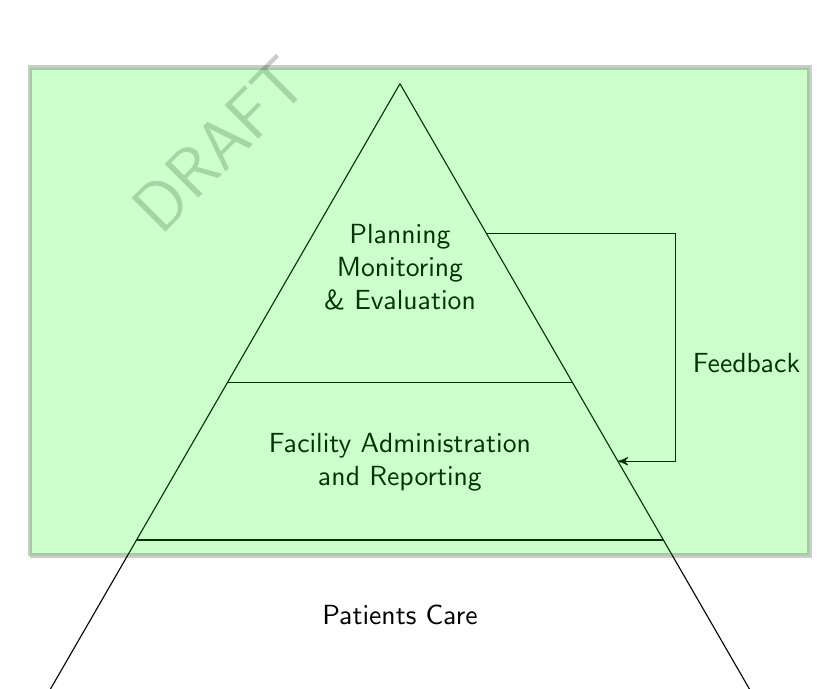
\begin{tikzpicture}[node distance=2cm]
\coordinate (A) at (-4.5,0) {};
\coordinate (B) at ( 4.5,0) {};
\coordinate (C) at ( 0,7.7942) {};
\draw[name path=AC] (A) -- (C);
\draw[name path=BC] (B) -- (C);
\draw (1.1,5.8971)--(3.5,5.8971) ;
\draw(3.5,5.8971)--(3.5,3) ;
\draw [->](3.5,3)--(2.77,3) ;
\node at (4.4,4.25) {Feedback};
\foreach \y/\A/\txtHigh in {0/Patients Care/0.8 ,2/Facility Administration \\ and Reporting/2.5,4/Planning \\ Monitoring \\ \& Evaluation /4.8}{
    \path[name path=horiz] (A|-0,\y) -- (B|-0,\y);
    \draw[name intersections={of=AC and horiz,by=P},
          name intersections={of=BC and horiz,by=Q}] (P) -- (Q)
          node[align = center,above] at (0,\txtHigh){\A};
          }
    \filldraw[ultra thick, draw=black, fill=green, opacity=0.2] (-4.7,1.8) -- (-4.7,8) -- (5.2,8) -- (5.2,1.8) -- (-4.7,1.8) ;
\end{tikzpicture}
\end{minipage}
\caption{Objective four definition}
\label{Paper Four}
\end{figure}




Reflections on social conditions of HMIS data usage  / politics of administrative statistics.

Data is not produced to create knowledge, but to implement disciplinary monitoring. Thinking mainly in terms of indicators.

Case study : analyse de textes M\&E / projets de reforme de systemes hmis, et analyse de la vision des HMIS qu'ils proposent. quelle place pour la societe civile ? inversion des priorites.

    \subsection{Setting}

    \subsection{Data}

    \subsection{Analysis}

    \subsection{Timeline}


%%%%%%%%%%%%%%%%%%%%%%%%%%%%%%%%%%%%%%%%%%%%%%%%%%%
%% 			BIBLIOGRAPHY
%%%%%%%%%%%%%%%%%%%%%%%%%%%%%%%%%%%%%%%%%%%%%%%%%%%
%\cleardoublepage
%\phantomsection\addcontentsline{toc}{section}{Références}
\newpage
\bibliography{bibliographie}


\end{document}
